\documentclass{ctexart}
\usepackage{xeCJK}
%\setCJKmainfont{AR PL UKai CN}
%\setCJKmainfont{AR PL UKai}
\usepackage{geometry}
\usepackage{caption}
\usepackage{graphicx, subfig}
\geometry{a4paper,left=4cm,right=4cm}
\usepackage{appendix}
\usepackage{amsmath}
\usepackage{amssymb,color}
\usepackage[colorlinks,linkcolor=blue,anchorcolor=blue,citecolor=red]{hyperref}
\usepackage{slashed}
\usepackage{simplewick}
\usepackage{tikz}
\usepackage{tcolorbox}
%colors
\def\blacktext#1{{\color{black}#1}}
\def\bluetext#1{{\color{blue}#1}}
\def\redtext#1{{\color{red}#1}}
\def\darkbluetext#1{{\color[rgb]{0,0.2,0.6}#1}}
\def\skybluetext#1{{\color[rgb]{0.2,0.7,1.}#1}}
\def\cyantext#1{{\color[rgb]{0.,0.5,0.5}#1}}
\def\greentext#1{{\color[rgb]{0,0.7,0.1}#1}}
\def\darkgray{\color[rgb]{0.2,0.2,0.2}}
\def\lightgray{\color[rgb]{0.6,0.6,0.6}}
\def\gray{\color[rgb]{0.4,0.4,0.4}}
\def\blue{\color{blue}}
\def\red{\color{red}}
\def\green{\color{green}}
\def\darkgreen{\color[rgb]{0,0.4,0.1}}
\def\darkblue{\color[rgb]{0,0.2,0.6}}
\def\skyblue{\color[rgb]{0.2,0.7,1.}}
%%control
\def\be{\begin{equation}}
\def\ee{\nonumber\end{equation}}
\def\beq{\begin{equation}}
\def\eeq{\end{equation}}
\def\bea{\begin{eqnarray}}
\def\eea{\end{eqnarray}}
\def\bmat#1{\left(\begin{array}{#1}}
\def\emat{\end{array}\right)}
\def\bcase#1{\left\{\begin{array}{#1}}
\def\ecase{\end{array}\right.}
\def\bmini#1{\begin{minipage}{#1\textwidth}}
\def\emini{\end{minipage}}
\def\tbox#1{\begin{tcolorbox}#1\end{tcolorbox}}
\def\pfrac#1#2#3{\left(\frac{\partial #1}{\partial #2}\right)_{#3}}
%%symbols
\def\bropt{\,(\ \ \ )}
\def\sone{$\star$}
\def\stwo{$\star\star$}
\def\sthree{$\star\star\star$}
\def\sfour{$\star\star\star\star$}
\def\sfive{$\star\star\star\star\star$}
\def\rint{{\int_\leftrightarrow}}
\def\roint{{\oint_\leftrightarrow}}
\def\stdHf{{\textit{\r H}_f}}
\def\deltaH{{\Delta \textit{\r H}}}
\def\ii{{\dot{\imath}}}
\def\skipline{{\vskip0.1in}}
\def\skiplines{{\vskip0.2in}}
\def\lagr{{\mathcal{L}}}
\def\hamil{{\mathcal{H}}}
\def\vecv{{\mathbf{v}}}
\def\vecx{{\mathbf{x}}}
\def\vecy{{\mathbf{y}}}
\def\veck{{\mathbf{k}}}
\def\vecp{{\mathbf{p}}}
\def\vecn{{\mathbf{n}}}
\def\vecA{{\mathbf{A}}}
\def\vecP{{\mathbf{P}}}
\def\vecsigma{{\mathbf{\sigma}}}
\def\hatJn{{\hat{J_\vecn}}}
\def\hatJx{{\hat{J_x}}}
\def\hatJy{{\hat{J_y}}}
\def\hatJz{{\hat{J_z}}}
\def\hatj#1{\hat{J_{#1}}}
\def\hatphi{{\hat{\phi}}}
\def\hatq{{\hat{q}}}
\def\hatpi{{\hat{\pi}}}
\def\vel{\upsilon}
\def\Dint{{\mathcal{D}}}
\def\adag{{\hat{a}^\dagger}}
\def\bdag{{\hat{b}^\dagger}}
\def\cdag{{\hat{c}^\dagger}}
\def\ddag{{\hat{d}^\dagger}}
\def\hata{{\hat{a}}}
\def\hatb{{\hat{b}}}
\def\hatc{{\hat{c}}}
\def\hatd{{\hat{d}}}
\def\hatN{{\hat{N}}}
\def\hatH{{\hat{H}}}
\def\hatp{{\hat{p}}}
\def\Fup{{F^{\mu\nu}}}
\def\Fdown{{F_{\mu\nu}}}
\def\newl{\nonumber \\}
\def\vece{\mathrm{e}}
\def\calM{{\mathcal{M}}}
\def\calT{{\mathcal{T}}}
\def\calR{{\mathcal{R}}}
\def\barpsi{\bar{\psi}}
\def\baru{\bar{u}}
\def\barv{\bar{\upsilon}}
\def\qeq{\stackrel{?}{=}}
\def\torder#1{\mathcal{T}\left(#1\right)}
\def\rorder#1{\mathcal{R}\left(#1\right)}
\def\contr#1#2{\contraction{}{#1}{}{#2}#1#2}
\def\trof#1{\mathrm{Tr}\left(#1\right)}
\def\trace{\mathrm{Tr}}
\def\comm#1{\ \ \ \left(\mathrm{used}\ #1\right)}
\def\tcomm#1{\ \ \ (\text{#1})}
\def\slp{\slashed{p}}
\def\slk{\slashed{k}}
\def\calp{{\mathfrak{p}}}
\def\veccalp{\mathbf{\mathfrak{p}}}
\def\Tthree{T_{\tiny \textcircled{3}}}
\def\pthree{p_{\tiny \textcircled{3}}}
\def\dbar{{\,\mathchar'26\mkern-12mu d}}
\def\erf{\mathrm{erf}}
\def\const{\mathrm{constant}}
\def\pheat{\pfrac p{\ln T}V}
\def\vheat{\pfrac V{\ln T}p}
%%units
\def\fdeg{{^\circ \mathrm{F}}}
\def\cdeg{^\circ \mathrm{C}}
\def\atm{\,\mathrm{atm}}
\def\angstrom{\,\text{\AA}}
\def\SIL{\,\mathrm{L}}
\def\SIkm{\,\mathrm{km}}
\def\SIyr{\,\mathrm{yr}}
\def\SIGyr{\,\mathrm{Gyr}}
\def\SIV{\,\mathrm{V}}
\def\SImV{\,\mathrm{mV}}
\def\SIeV{\,\mathrm{eV}}
\def\SIkeV{\,\mathrm{keV}}
\def\SIMeV{\,\mathrm{MeV}}
\def\SIGeV{\,\mathrm{GeV}}
\def\SIcal{\,\mathrm{cal}}
\def\SIkcal{\,\mathrm{kcal}}
\def\SImol{\,\mathrm{mol}}
\def\SIN{\,\mathrm{N}}
\def\SIHz{\,\mathrm{Hz}}
\def\SIm{\,\mathrm{m}}
\def\SIcm{\,\mathrm{cm}}
\def\SIfm{\,\mathrm{fm}}
\def\SImm{\,\mathrm{mm}}
\def\SInm{\,\mathrm{nm}}
\def\SImum{\,\mathrm{\mu m}}
\def\SIJ{\,\mathrm{J}}
\def\SIW{\,\mathrm{W}}
\def\SIkJ{\,\mathrm{kJ}}
\def\SIs{\,\mathrm{s}}
\def\SIkg{\,\mathrm{kg}}
\def\SIg{\,\mathrm{g}}
\def\SIK{\,\mathrm{K}}
\def\SImmHg{\,\mathrm{mmHg}}
\def\SIPa{\,\mathrm{Pa}}


%\cpic{<尺寸>}{<文件名>}}用于生成居中的图片。
\newcommand{\cpic}[2]{
\begin{center}
\includegraphics[scale=#1]{#2}
\end{center}
}

%\cpicn{<尺寸>}{<文件名>}{<注释>}用于生成居中且带有注释的图片,其label为图片名。
\newcommand{\cpicn}[3]
{
\begin{figure}[H]
\cpic{#1}{#2}
\caption{#3\label{#2}}
\end{figure}
}
\title{实验D5 CCD原理与应用}
\begin{document}
\maketitle

\begin{tabular}{|p{8em}|p{8em}|p{8em}|p{5em}|}
\hline
		\large{实验方案} &\large{实验记录}  &\large{分析讨论} &\large{总成绩}\\
		\hline
		        &          &          &  \\
	    \hline
	\hline 
	年级、专业: &17级物理学 &组号:& 6 \\
	\hline
	姓名:& 徐昊霆 &学号:&17353071  \\
	\hline
	日期:& 2019.9 &教师签名: &  \\
    \hline	
        \end{tabular}
        
        1. 实验报告由三部分组成:
        
        1) 预习报告:(提前一周)认真研读实验讲义,弄清实验原理;实验所需的仪器设备、用具及其使用(强烈建议到实验室预习),完成讲义中的预习思考题;了解实验需要测量的物理量,并根据要求提前准备实验记录表格(由学生自己在实验前设计好,可以打印)。预习成绩低于50\%者不能做实验(实验D2和D3需要提前一周的周四完成预习报告交任课老师批改,批改通过后,才允许做实验)。
        
        2) 实验记录:认真、客观记录实验条件、实验过程中的现象以及数据。实验记录请用珠笔或者钢笔书写并签名(用铅笔记录的被认为无效)。保持原始记录,包括写错删除部分,如因误记需要修改记录,必须按规范修改。(不得输入电脑打印,但可扫描手记后打印扫描件);离开前请实验教师检查记录并签名。
        
    3) 分析讨论:处理实验原始数据(学习仪器使用类型的实验除外),对数据的可靠性和合理性进行分析;按规范呈现数据和结果(图、表),包括数据、图表按顺序编号及其引用;分析物理现象(含回答实验思考题,写出问题思考过程,必要时按规范引用数据);最后得出结论。
    实验报告就是预习报告、实验记录、和数据处理与分析合起来,加上本页封面。
    
    2. 每次完成实验后的一周内交实验报告。
    
    3. 实验报告建议双面打印。
\newpage
\tableofcontents
\newpage
\section{实验原理与方案}
\subsection{实验目的}
1. 了解CCD的构造,工作原理和应用。

2. 掌握二相线阵CCD和隔行转移面阵CCD的驱动脉冲波形及其特性测量,并理解各驱动
脉冲在电路中的作用和电荷转移过程。

3. 掌握线阵CCD和面阵CCD非接触测量物体尺寸和角位置的基本原理和方法,并能自主
设计符合特定要求的测量方案。

4. 熟悉CCD图像数据采集软件的基本操作,掌握图像数据采集和初步的图像处理技术
如点运算、彩色图像分解、颜色识别等。

\subsection{实验安全注意事项}
在 CCD 应用技术实验前,为了保障人身安全,避免设备损坏,并且达到实验目的,实验
人员需要注意以下安全事项:

(1) 要爱护实验仪器和示波器、计算机等实验设备,不允许将其它不相关的仪器在未
经许可的情况下与实验仪进行连接。

(2) 所有仪器设备必须轻拿轻放,避免碰撞掉落造成损坏。

(3) 激光功率不宜调至过大,同时避免对准眼睛照射。

(4) 不能用手直接接触准直镜和反射镜镜片。

(5) 用示波器测量 CCD 特性时,黑色线要接地线。

(6) 实验完成后,按实验前原样复原仪器设备。

\subsection{仪器用具}
\begin{tabular}{c|c|c|c}
	\hline
        编号 & 仪器名称 &数量& 主要参数(型号,测量范围,精度) \\
	\hline 
	1 &  实验机箱&1 &\\
        2 &  90mm导轨&1 & RL-POR01,90mm 宽,30mm 高,
600mm 长\\
        3 & 90mm 滑块 &1&RL-RC01,120mm 宽,40mm 长\\
        4 & 90mm 旋转滑块  &1&RL-RC02-R,120mm 宽,65mm 长,旋转\\
        5 &  调节套筒 &1&RL-PH01,L51mm\\
        6 & 调节套筒 &1&RL-PH02,L76mm\\
        7 &  支杆 &1&RL-PO02,L51mm,双头阳螺纹\\
        8 &  支杆 &1&RL-PO02,L76mm,双头阳螺纹\\
        9&  激光管夹持器 &1&RL-LH01,Φ25~Φ50mm,V 型\\
        10 &  光纤准直镜 &1&RL-CL11,通光 Ф1mm,接口 FC/PC\\
        11 &  光纤准直镜 &1&RL-CL51,通光 Ф30mm,接口 FC/PC\\
        12&  光纤耦合半导体激光器 &1&650nm,2mW,功率可调\\
        13&  相机防尘盖 &1&C接口\\
        14 &  电源线 &1&三相电源线,220V\\
        15&  DC电源线 &1&双头DC插头\\
        16&  USB线 &1&A公口转B公口\\
        17&  USB线 &1&A-B口,CMOS相机用\\
        18 &  面阵CCD组件 &1&RL-CC01,C 接口,集成测试端子USB 端口输出\\
        19 &  线阵 CCD 组件 &1&RL-CC02,M52 接口,USB 输出\\
        20 &  BNC-2mm 信号测试线 &2&1 头 BNC,另外 2 头是 2mm 标准插头\\
        21 &  被测工件 &1&两种直径测试标准件 $\Phi$10,$\Phi$12\\
        22 &  软件光盘 &1&CCD实验线阵部分\\
        23&  透镜/发射镜支架 &1&JT-JJ01,$\Phi$45 内孔,可装 $\Phi$20,$\Phi$25.4,$\Phi$30,$\Phi$40mm 的镜片\\
        24 &  镜圈 &1&JT-JQ40,外径 $\Phi$45mm,装 $\Phi$40mm镜片\\
        25 & 磁性表座 &1&RL-MB01,外形 61x51x55mm,吸力45kg\\
        26&  高亮度LED照明光源 &1&白色\\
        27 &  白屏(带刻度) &1&RL-LED01-W,白色\\
        28 &  加强铝反射镜 &1&MIR0101,Φ40x4mm,装在透镜/反射镜座\\
        29 &  钢尺 &1& 500mm\\
        30& LED可调电源 &1&9V输出 \\
        31& 干版夹 &1& JT-GB01,外形 60x26x24mm\\
        32& 变焦镜头 &1& EV0410MC.HR,1/2”,f4~12mm,F1.6 \\
        33&颜色检测卡纸&1&和白屏夹至干板夹反面\\
        34&H 型被测物&1&和白屏夹至干板夹正面 \\
	\hline        
\end{tabular}
\subsection{实验背景}
\subsubsection{CCD简介}
电荷耦合器件(Charge Coupled Devices,简称为 CCD),是 70 年代初期发现的新型
集成光电传感器件,可直接将光学信号转换为模拟电流信号,电流信号经过放大和模数转换,
实现图像的获取、存储、传输、处理和复现。其显著特点是:1.体积小重量轻;2.功耗小,
工作电压低,抗冲击与震动,性能稳定,寿命长;3.灵敏度高,噪声低,动态范围大;4.响
应速度快,有自扫描功能,图像畸变小,无残像。自发现以来,CCD 及其技术迅速发展,已
广泛应用在科技、军事、教育、医学、工业等领域,是图像采集和数字化的关键器件。

CCD 主要有线阵列和面阵列两种基本类型,各有不同的工作原理与特性。线阵 CCD 由于
工作原理简单,易于掌握,通常用于工业领域的非接触自动检测设备上,尤其是自动化生产
过程或生产线上用作在线非接触光电检测设备,主要检测物体的尺寸、运动速度、加速度、
运动规律、位置、面形、粗糙度、变形量、光学特性变化、条码信息和其他应用。而面阵 CCD
又称全幅式 CCD,阵列型 CCD。相比线阵 CCD,它的优点是可以获取二维图像信息,测量图
像直观,是工业相机、数码相机、摄像机等系统的核心器件,广泛应用于面积、形状、尺寸、位置、甚至温度等的测量。面阵 CCD 有行间转移(IT)型、帧间转移(FT)型和行帧间转移(FIT)型三种。
\subsubsection{CCD结构与原理}
CCD 主要由感光部分、转移存储和移位输出控制等部分组成。CCD 的感光
部分叫做光(像) 敏单元,光敏单元是光电二极管或 MOS 或 CMOS 的阵列,光敏单元一般加有
电压,用以控制光敏单元的电容,由于有电容属性,因而可以存储电荷。光照射到光敏单元
产生电子-空穴对,电子-空穴对存储在光敏单元中。存储的电荷在一定时间后转移到移位寄
存器,移位寄存器为 MOS 结构,MOS 的电容可以存储电荷。相邻 2 次电荷转移的时间间隔称
为积分时间,由于电荷的转移时间很短,因此一般认为电荷转移的周期便是积分时间,积分
时间也就是光敏单元接受光照的时间。CCD 的移位寄存器的 MOS 结构有挡光层,因此不能产
生电子-空穴对。移位寄存器上加有驱动脉冲信号,使存储的电荷按一定次序串行输出。

CCD 成像原理可以简述为以下几个步骤:

(1) 对 MOS 金属栅电极施加时钟脉冲,则对应栅电极下半导体内形成可储存少数载流
子的 势阱 。

(2) 用光注入的方法,即当光线照射到 CCD 上,光电二极管受到光线的激发释放出信号
电荷,并输入势阱,实现信号电荷存储。

(3) 然后周期性地改变 时钟脉冲 的 相位 和幅度,势阱深度则随时间相应地变化,从而使注入的信号电荷在半导体内作定向转移。

(4) 信号电荷统一输出到放大器,经过放大和滤波后,由 A/D 将模拟电信号转换为数字
信号,即图像数据。

(5) 最后将这些图像数据进行读出、处理和存储,从而实现 CCD 成像。

\subsubsection{CCD的应用}
从 CCD 工作原理可以看出,CCD 具有光电转换、信号存储及信号传输能力,是一种崭新
的全固体自扫描成像器件。固体成像、信号处理和大容量存储器是 CCD 的三大主要用途。各
种线阵、面阵像感器已成功地用于天文、遥感、传真、卡片阅读、光测试和电视摄像等领域,
微光 CCD 和红外 CCD 在航遥空感、热成像等军事应用中显示出很大的作用。CCD 信号处理兼
有数字和模拟两种信号处理技术的长处,在中等精度的雷达和通信系统中得到广泛应用。
CCD 还可用作大容量串行存储器,其存取时间、系统容量和制造成本都介于半导体存储器和磁盘、磁鼓存储器之间。
\subsection{实验原理}
1. 两款 CCD 芯片结构与原理
本实验主要采用东芝 TCD1208AP 二相线阵 CCD 芯片和索尼 ICX409AK 面阵 CCD 芯片。
首先了解下这两款芯片结构及原理。
(1) 东芝 TCD1208AP 二相线阵 CCD 芯片
TCD1208AP 是一款 5V 供电的高灵敏度、低暗电流的二相线阵图
像传感器。其外形如右图所示,它包括 2160 个有效像敏单元,每个
像敏单元大小为 $14\SImum$(即像敏单元中心间距)。它的基本结构原理
图如图 3 所示,由 2212 个 PN 结光电二极管构成光敏元阵列,其中
前 40 个和后 12 个是用作暗电流检测而被遮蔽的,
中间 2160 个光电二极管是曝光像敏单元,
故一行完整的信号输出有 2160 个像元。每个光敏单元尺寸为 $14\SImum \times 14\SImum$,中心间距也是
14$\SImum$。光敏元阵列总长 30.24mm,光敏单元两边是转移栅,最外边是模拟转移寄存器,其输出部分由信号输出单元和补偿单元构成。

TCD1208AP 工作时主要由四路时序脉冲控制:SH,$\Phi1,\Phi 2$ 和 RS,其中 SH 是转移栅脉
冲,$\Phi 1,\Phi 2$ 是模拟转移寄存器驱动脉冲,RS 是复位脉冲。其时序脉冲如下图 4 所示,当
SH 高电平来到时,$\Phi 1$为高电平,Φ2 为低电平($\Phi 1$,Φ2 相互为互补时序脉冲)。CCD 模
拟转移寄存器中所有 $\Phi 1$ 电极下均形成深势阱,同时 SH 的高电平使 $\Phi 1$ 电极下的深势阱与
MOS 电容存储势阱(转移栅)沟通,MOS 电容中的信号电荷包通过转移栅转移到模拟移位寄
存器的 $\Phi 1$电极下的势阱中。当 SH 由高变低时,SH 低电平形成势垒,使 MOS 电容与 $\Phi 1$电
极隔离。而后,$\Phi 1$与 $\Phi 2$交替变化,模拟移位寄存器在 $\Phi 1$ 与 $\Phi 2$ 脉冲的作用下驱使 $\Phi 1$
电极下势阱中的信号电荷向左移动,并经输出电路由 OS 电极输出。RS 是复位输出级的复位脉冲,复位一次输出一个光脉冲信号。

(2) 索尼 ICX409AK 面阵 CCD 芯
ICX409AK 是一款隔行转移型面阵 CCD 芯片,可用于 PAL 制式彩
色电视机摄像系统。它的总像素单元数为 795(H)×596(V),有效
像元数为 752(H)$\times$582(V),像元尺寸为 6.50$\SImum (H) × 6.25\SImum$
(V),像敏区的总面积为 5.59mm (H) $\times$ 4.68mm (V),封装在 14 脚
的 DIP 标准管座上,其外形尺寸如右图所示。
ICX409AK 的原理结构图如图 5 所示,它由光电二极管阵列、垂直 CCD 移位寄存器及水
平 CCD 模拟移位寄存器三部分构成。图 6、图 7 为 ICX409AK 的垂直同步脉冲和水平同步脉
冲时序图,从图中可以看出,在场消隐期间,V1~V4 及 H1、H2 上所加的脉冲均属于均衡脉
冲,V1、V2 为正脉冲,使光积分电极完成光积分。在场消隐期间,V1 和 V3 的正脉冲完成信
号由光积分区向垂直移位寄存器转移。转移完成后经过两个行周期的转移进入有效像元信号
的输出。在行消隐期间,V1 中的信号在 V1 下降沿倒入 V2,V2 的下降沿倒入 V3,V3 的下降
沿倒入 V4,V4 的下降沿倒入 H1。在行正程期间,V1~V4 保持不变,倒入到水平移位寄存器
中的信号在水平脉冲的作用下,一个个从 CCD OUT 端输出。

2. 驱动脉冲与积分时间关系
CCD 的输出信号受驱动频率和积分时间共同决定,如图 8 所示。驱动频率影响输出信号
的频率,积分时间影响帧速率。积分时间的改变本质上是通过增加或减少驱动脉冲来实现的。
驱动脉冲频率上限受电荷自身转移时间限制,当工作频率升高时,若电荷本身从一个电极转
移到另一个电极所需要的时间 t 大于驱动频率使其转移的时间 T/3,那么,信号电荷跟不上
驱动脉冲的变化,将会使转移效率大大下降。SH 脉冲在高电平时沟通像敏单元和模拟转移
寄存器,使像敏单元中的光电子转移到模拟转移寄存器。相邻两个 SH 脉冲之间的时间就是
像敏单元的感光时间,这里称为积分时间。模拟转移寄存器中的光电荷的输出时间应该小于
积分时间才能保证光电信号的完整。因此,积分时间长短由两个条件决定,一是足够感光,
二是传输完成。

3. 投影成像测量法
投影成像测量法主要适用于测量与 CCD 传感面的尺寸相当的物体的尺寸。如图 9 所示,
此方法利用一束平行光照射在被测物体上,最终投影在 CCD 的传感面上,被测物的尺寸可以
通过计算 CCD 上产生的阴影宽度获得,只要数据采集系统计算出阴影部分像元个数与像元
尺寸的乘积就得到了被测物体的尺寸,这里假设平行光是理想的。投影法的测量精度由平行
光的准直性和 CCD 像元尺寸决定。但是,平行光准直度很难达到理想情况,因此还需要用算
法对测量值进行修正,对尺寸进行标定来使得测量结果准确。

4. 角位置测量法
角位置测量的方法有多种,通常采用专用的角位置传感器,如旋转变压器、圆感应同步
器,圆光栅等,在一些特定的条件下,如没有转动机构的情况下,需要进行角位置测量时,
可以采用 CCD 传感器进行位置测量,通过光学换算可以将 CCD 的像素尺寸转换到反射镜的
旋转角位置上。这种光电测量法是一种高精度、高可靠性、成本低的非接触式测量方法,可
以实现小角度的静态和动态测量。

测角系统的工作原理如图 10 所示,反射镜的转动量转换为激光光束角度的变化,反射
光束照射到线阵 CCD 探测器上,CCD 首先完成光电转换,即产生与入射的光辐射量成线性关
系的光电荷。然后在 CCD 驱动脉冲的控制下,将电荷移位至输出电路,经输出电路将电荷量
转化为电压量输出。这样在 CCD 芯片的输出端就产生了与光电荷量成正比的弱电压信号,经
过滤波、放大处理,通过驱动电路输出一个能表示敏感物体光强弱的电信号或标准的视频信
号。将一维光学信息转变为电信息输出,后端的放大和 A/D 转换电路将信息转换为数字量,
将数字量利用 USB 接口传输至计算机,通过上位机软件计算出转动的角度量。当反射镜绕图中 O 点转动,只要检测出光斑在 CCD 上移动距离即可得到旋转轴的旋转角度,由此,线阵
CCD 就可以实现角位置测量功能。

5. 模拟/数字信号转换基本原理及 USB 数据传输
本系统用到的数据采集板主要包括信号调理、AD 转换和 USB 数据传输。信号调理主要
是放大 CCD 信号,使之满足 AD 转换器的输入要求,电路结构简单,因此,这里简单介绍 ADC
的基本原理和 USB 数据传输。ADC 模拟/数字转换过程可以用图 11 表示,主要有两个步骤,
首先对欲转换的数据进行取样和保存,然后再将获取到的数据加以量化,如此就完成了数据
的转换。其中取样的目的在于将原始模拟数据一一撷取,因此取样率越高信号越不容易失真,
即分辨率越高;量化的目的则是将由取样所获得的数据以 0 与 1 的组合予以编码,同样的量
化位数越高则分辨率越高。

USB 数据传输采用的接口具有数据传输速度快、兼容性强、即插即用等优点,已经广泛
应用于数据传输、图像采集领域。相比于过去的老式接口,其数据传输速率非常快,最高可
达 480Mbps,可以满足教学实验的要求。USB 的结构包含四种基本的数据传输类型:控制数
据传送、批量数据传送、中断数据传送、同步数据传送,不同的传输方式适合不同类型的数
据,在应用中要根据实际情况选择合适的传输方式。

6. 图像处理方法 --- 二值化
在不要求图像灰度的系统中,为提高处理速度和降低成本,我们往往采用二值化图像处
理方法。二值化处理是把图像和背景作为分离的二值(0,1)对待。光学系统把被测物体成
像在 CCD 光敏像元上。由于被测物与背景在光强上的变化反映在 CCD 视频信号中所对应的
图像尺寸边界处会有明显的电平变化,通过二值化处理把 CCD 视频信号中图像尺寸部分与
背景部分分离成二值电平。二值化处理方法很多,有固定阈值法、浮动阈值法和微分法等,
我们这里从硬件上实现固定阈值法。固定阈值法是一种最简便的二值化处理方法。将线阵 CCD 输出的视频信号送入电压比较器
的同相输入端,比较器的反响输入端加可调的电平就构成了固定阈值二值化电路。当 CCD 视
频信号的幅度稍稍大于阈值电压(电压比较器反相输入端的电位)时,电压比较器输出为高
电平;CCD 视频信号小于等于阈值电压时,电压比较器输出为低电平。CCD 信号经电压比较
器后输出的是二值化方波信号。调节阈值电压,方波脉冲的前、后将发生移动,脉冲的宽度
发生变化。当 CCD 视频信号输出含有被测物体直径的信息时,可以通过适当调节阈值电压获
得方波脉冲宽度与被测物体直径的精确关系。

7. 图像处理方法 --- 点运算
数字图像处理技术的内容非常丰富(如图像的增强、图像压缩、图像还原、图像的相关
识别等等),处理方法也很多。它牵涉到许多数学变换问题(如图像的傅立叶变换、离散余
弦变换、沃尔什变换、哈得玛变换、斯拉特变换等)(详细内容请参见《光电图像处理》)。
这样复杂的技术问题不可能用一个实验解决,但是为增强学生对数字图像处理技术的认识,
我们从图像图形处理技术的基本处理方法—点运算开始,逐步学习数字图形图像的处理技
术。

(1)点运算的定义。对于一幅输入图像,将产生一幅输出图像,输出图像的每个像素
点的灰度值由输入图像的像素点决定。点运算由灰度变换函数(gray-scale transformation,
GST)决定。

(2)灰度直方图。灰度直方图是数字图像处理技术中一个最简单、最有用的工具,它
描述了一幅图像的灰度级内容。任何一幅图像的直方图都包括了可见的信息,某些类型的图像还可用其直方图进行描述。灰度直方图是灰度的函数,它描述的是图像中具有该灰度值的像素个数,其横坐标表示像素的灰度级别,纵坐标是该灰度出现的频率(像素个数)。可以根据具体实验观察并分析典型图像的直方图。

(3)灰度的线性变换。灰度的线性变换是点运算中最简单的运算之一。灰度的线性变
换是将图像中所有点的灰度按照线性灰度变换函数进行变换。
该线性灰度变换函数为 $f (x)$,是一维的线性函数
\beq
f(x) = f_A x + f_B
\eeq
上式中 $x$ 自变量为灰度值, $f_A$ 为线性函数的斜率, $f_B$ 为线性函数的截距,均为非定值常量。
当 $f_A >1$ 时,输出图像的对比度将增大;当 $f_A <1$ 时,输出图像的对比度将减小;当 $f_A =1$
且$f_B \ne 0$ 时,变换仅使所有像素的灰度值上移或下移,其效果是使整个图像更暗或更亮;如
果 $f_A <0$,暗区域将变亮,亮区域将变暗,点运算完成图像求补运算。特殊情况下,当 $f_A=1$, $f_B =0$ 时,输出图像和输入图像相同;当 $f_A =-1$, $f_B =255$ 时,输出图像的灰度正好反转。

(4)灰度的阈值变换。灰度的阈值变换可以将一幅灰度图像转换成黑白二值图像的变
换。灰度的二值化变换是将一幅灰度图像转化成黑白二值图像。具体操作过程是先由用户设
定一个阈值 $T_{th}$ ,如果图像中某像素单元的灰度值小于该阈值,则该像素单元的灰度值变换为 0,否则,其灰度值为 255。变换函数为
\bea
f(x) &=& 0\,  x<T_{th} \\
&=& 255  \, x\le T_{th}
\eea
灰度的窗口变换也是常见的点运算。它的操作和阈值变换类似。该变换过程是先设置窗口$(L\le x \le U)$, $x$ 值小于下限 $L$ 的像素单元的灰度值变换为 $0$,大于上限 $U$ 的像素单元的灰度值变换为 255,而处于窗口中的灰度值保持不变。灰度窗口变换函数为
\bea
f(x) &=& 0  \,\,\,\, x<L \\
&=& x \, \,\,\,\, L\le   x\le U \\
&=& 255 \,\,\,\, x\ge U
\eea

(5)灰度拉伸变换。灰度拉伸变换与灰度的线性变换类似,都用到了灰度的线性变换。
不同之处在于灰度拉伸变换并不是完全的线性变换,而是分段线性变换。它的变换函数为图中两个转折点的坐标。
\bea
f(x) &=& \frac{y_1}{x_1}x    \,\,\,\,\,x<x_1 \\
&=& \frac{y_2-y_1}{x_2-x_1}(x_2-x_1) + y_1 \,\,\,\,\,x_1<x<x_2\\
&=& \frac{225-y_2}{225-x_2}(x - x_2) + y_2\,\,\,\,\, x>x_2
\eea

(6)灰度均衡变换,灰度均衡变换有时也称直方图均衡变换,它能使输入图像转换为
在新图像每一灰度级上都有相同的像素点数的输出图像。灰度均衡变换的原理式如下
\beq
A[a] = \left(\sum_{i = 0}^a  N[i]\right)\times 225 /(H\cdot W)
\eeq
式中 $a$ 为原图像像素灰度值(0-255),经过灰度均衡运算 $a$ 的值变为灰度均衡值 $A,N$ 为原图像各灰度值对应的像元数量,$H$ 为图像的高度(单位是像元数),W 为图像的宽度(单位是像元数)。例如原图像像元灰度值为 20 的像素点,经灰度均衡变换后,灰度变为
\beq
A[20] = \left(\sum_{i = 0}^{20}  N[i]\right)\times 225 /(H\cdot W)
\eeq
经过灰度均衡后,图像的对比度大大提高,转换后图像的灰度分布也趋于均匀。

8. 彩色图像处理方法
在用彩色面阵 CCD 获取被测对象的表面特征时,由于对象物体具有不同的色彩,因此学
习利用彩色面阵 CCD 进行彩色图像的分解与合成,进而用此种方法对颜色信息进行识别和
图像处理至关重要。对于彩色图像,它的显示来源于 R、G、B 三原色亮度的组合。针对目标
的单色亮度、对比度,可以人为的分为“0~255”,共 256 个亮度等级。“0”级表示不含有
此单色,“255”级表示最高的亮度,或此像元中此色的含量为 100\%。根据 R、G、B 的不同
组合,就能表示出 256×256×256(约 1600 万)种颜色。当一幅图像中的每个像素单元被
赋予不同的 R、G、B 值,就能显示出五彩缤纷的颜色,形成彩色图像。通过彩色图像的处理
能提高原图像的质量。进一步的了解可看“彩色三要素”、“三基色原理”、“混色原理”、颜色的度量和表示”、“CIE 标准色度学系统”等基础知识。
\subsection{实验前思考题}
1. MOS 电容器工作原理是什么?

更详细的介绍请看参考文献~\cite{MOS}。MOS电容器是所有MOS(金属-氧化物-半导体)结构中最简单的,它是CCD的构成基础。MOS电容器有两种类型:表面沟道和埋沟。这两种类型MOS电容器的制造只有微小的不同。然而,由于埋沟电容结构具有很多显著的有点,因此这种结构成了CCD制造工艺的首选。事实上今天制造的所有CCD几乎都用了埋沟结构。

埋沟电容是一个p-型衬底上建造的;在p-型衬底表面上形成一个n-型区(1微米厚);然后,生长出一层薄的二氧化硅(0.1微米厚);再在二氧化硅层上用金属或高掺杂的多晶硅制作电极或者栅极;至此完成了MOS电容的制作。无偏置时,n-型层内含有多余的电子同p-型层扩散,p-型层内含有多余的空穴并向n-型层扩散;这个结构与二极管的结构完全相同。上述的扩散内部形成了内部电场,在n-型层内电势达到最大。

CCD曝光时,产生光生电荷,光生电荷在势阱里收集。随着电荷的增加,电势将逐渐变低,势阱被逐渐填满,不再能收集点和,达到饱和。

2. 光电转换的物理原理是什么?

光电转换过程的原理是光子将能量传递给电子使其运动从而形成电流。这一过程原则上需要用狄拉克方程来描述
\beq
\frac{1}{i}\gamma^{\mu}\partial_{\mu}\psi + m\psi = 0
\eeq

3. CCD 驱动脉冲是如何实现信号电荷转移和输运的?

具体的介绍详见~\cite{maichong}。 CCD的移位寄存器是一列排列紧密的MOS电容器,它的表面由不透光的铝层覆盖,以实现光屏蔽。 MOS电容器上的电压愈高,产生的势阱愈深,当外加电压一定,势阱深度随阱中的电荷量增加而线性减小.利用这一特性,通过控制相邻MOS电容器栅极电压高低来调节势阱深浅.制造时将MOS电容紧密排列,使相邻的MOS电容势阱相互“沟通”.认为相邻MOS电容两电极之间的间隙足够小(目前工艺可做到0.2微米),在信号电荷自感生电场的库仑力推动下,就可使信号电荷由浅处流向深处,实现信号电荷转移。


\newpage
\section{实验步骤与记录}
\begin{tabular}{|p{8em}|p{8em}|p{8em}|p{8em}|}
	\hline 
	专业:     &Physics       &年级:      & 17     \\
	\hline
	姓名:& 徐昊霆 &学号:&17353071  \\
	\hline
	室温:&                    &实验地点 & 教学楼 \\
	\hline	
	学生签名: & & 评分: & \\
	\hline
	日期: & 2019.9.9 & 教师签名:&  \\
	\hline
\end{tabular}
\subsection{实验内容}
\subsubsection{线阵 CCD 驱动及其特性测量}
掌握用双踪迹示波器观测二相线阵 CCD 驱动脉冲的频率、幅度、周期和各路驱动脉冲
之间的相位关系等的测量方法;通过观测线阵 CCD 不同驱动脉冲频率、幅度、周期、延迟
等,掌握二相线阵 CCD 的基本工作原理,理解各驱动脉冲在电路中的作用,理解电荷转移
的过程。并且通过对线阵 CCD 在不同工作频率和不同积分时间情况下的输出信号的测量,
进一步掌握 CCD 的有关特性,
掌握积分时间的意义,
了解不同的驱动频率和积分时间对 CCD
输出信号的影响。

实验步骤:
(1) 打开线阵 CCD 实验箱,按实验装置图 13 安装仪器,并完成准直镜和线阵组件对
准。打开半导体激光器,功率调至最小,并使激光照射到线阵 CCD 相机;
(2) 用 12PIN 排线连接线阵 CCD 相机和测试面板,用 USB 连接线将线阵相机和计算
机连接起来并打开计算机电源。
(注意 CCD 相机与测试面板之间的 12PIN 线排针
孔对应)
;
(3) 打开示波器电源开关,
待预热后将测试笔 CH 1 接到测试面板板上的转移脉冲 SH 输
出端上,先仔细调节示波器的触发脉冲电平旋钮使示波器显示波形稳定,既表示示
波器已被 SH 同步,再调节示波器的扫描频率“旋钮”或“按键”
,使 SH 脉冲的
宽度适合观测,以能够观察到一个或二个周期为最佳,观察并记录转移脉冲 SH 的
频率和周期。同样的方法测试复位信号 RS;
(4) 将示波器测试笔 CH1 和 CH2 分别接至测试面板上的 Φ1,Φ2 测试孔,调节示波器
的电压刻度和扫描频率,以能同时看到两路测试信号,并且能够观察到一个或两个
周期为佳,观察并记录 Φ1,Φ2 信号之间的相位关系。
(5) 将测试笔 CH1 探头接 CCD 输出测试孔,观察并记录线阵 CCD 相机在光照和遮挡不同情况下的 CCD 输出端信号变化。
(6) 将示波器测试笔 CH 1 接到测试面板上标有二值化输出的测试孔,调节示波器扫描
频率和触发电平,使能看到完整一帧 CCD 输出信号为佳,并观察不同阈值电压下
CCD 二值化输出信号的变化。
(7) 运行线阵相机采集软件,点击采集按钮 “采集”
,观察遮挡线阵 CCD 不同部位采
集到的波形有何变化。
(8) 调节激光功率输出,使线阵 CCD 处于不饱和状态。
(9) 在准直镜和线阵 CCD 之间加入被测物,点击软件暂停按钮“暂停”
,移动频率设置
滑动条并点击设置按钮“设置”
,修改线阵 CCD 相机频率,观察线阵相机输出波形
的变化趋势,并记录变化规律;
(10) 点击软件暂停按钮“暂停”
,将频率设置滑动条移至最左端,移动积分时间设置滑
动条并点击设置按钮“设置”
,修改线阵 CCD 相机积分时间,观察线阵相机输出波
形的变化趋势,并记录变化规律。

要求: 测试端子 SH、RS、$\Phi$1、$\Phi$2 周期和频率记录下表,驱动脉冲波形利用示波器 USB 接口导出,作图,然后与图 4 中的 TCD1208AP 工作时序图比较。同时结合改变驱动频率和积分时间对 CCD 输出端波形变化趋势,分析线阵 CCD 工作原理。

\begin{tabular}{|p{5em}|p{5em}|p{5em}|p{5em}|p{5em}|}
	\hline 
	测试端子     &SH       &RS      & $\Phi 1$&$\Phi 2$     \\
	\hline
	周期($\mu \rm{s}$) &  & &  &  \\
	\hline
	频率(kHz)&        &            & &  \\
	\hline	
\end{tabular}


\subsubsection{利用线阵CCD测量工件直径和角位置}
线阵 CCD 的输出信号包含了 CCD 各个像元所接收光强度的分布和像元位置的信
息。利用线阵 CCD 可以获取被测对象的特征信息如尺寸和角位置。为了了解线阵 CCD
相机在工业上的应用,在掌握线阵 CCD 原理的基础上,下面我们通过测量被测物体的
直径和角度的两个例子,掌握非接触在线测量方法,并能自己设计符合要求的方案。

实验步骤:

a 工件直径测量实验
(1) 根据投影成像测量法原理搭建下图所示光路结构,将标准块放置于图中滚针位置。

(2) 打开线阵 CCD 相机测试,在物体输入文本框“物体宽度”中输入标准块宽度,点
击采集按钮,在图形显示区利用红色和蓝色辅助线采集标准块像素宽度,点击标定
按钮“标定”获得系统实际物理尺寸和像素之间的映射关系。

(3) 将标准块换成被测物体,调节半导体激光器输出功率,使线阵 CCD 相机工作在未
饱和状态,同时利用实验内容 1 记录的规律,设置最佳驱动频率和积分脉冲时间,
使得 CCD 输出波形凹槽清晰可见。

(4) 将辅助线置于物体边缘变化斜率最大的位置,利用辅助线获得被测物体宽度,点击计算物体宽度按钮“计算物体宽度”
,利用上述标定的实际尺寸和像素之间的映射
关系就可以得到物体的物理尺寸。

(5) 多次测量不同物体,获得多组数据,计算绝对误差,并分析误差来源。

$\phi 12$滚针直径测量数据

\begin{tabular}{|p{5em}|p{5em}|p{5em}|p{5em}|}
	\hline 
        测量次数 & 1& 2&3     \\
	\hline
	测量值 & & &  \\
	\hline
	误差 & & &  \\
	\hline	
\end{tabular}

$\phi 10$滚针直径测量数据

\begin{tabular}{|p{5em}|p{5em}|p{5em}|p{5em}|}
	\hline 
        测量次数 & 1& 2&3     \\
	\hline
	测量值 & & &  \\
	\hline
	误差 & & &  \\
	\hline	
\end{tabular}

b 角位置测量实验

(1) 搭建测量系统,半导体激光器、反射镜安装在导轨上,线阵 CCD 相机安装在磁座上,相互呈一定角度。

(2) 打开线阵 CCD 相机测试软件,打开半导体激光器电源,激光通过手动调节支杆上
的反射镜照射到线阵 CCD 光敏面,调节半导体激光器输出功率,使线阵 CCD 相
机工作在未饱和状态,
利用图形显示区的辅助线得到激光在线阵 CCD 上的位置 1。

(3) 手动调节反射镜角度,
注意防止角度过大导致反射光线超过线阵 CCD 光敏面长度,
在上位机测量激光光斑在 CCD 上的位置并记录。

(4) 得到光斑移动像素宽度,乘以像素大小 $14\SImum$,得到光斑移动的实际距离。光斑移
动实际距离除以线阵 CCD 相机到铝反射镜的距离,就得到反射镜转过的弧度,进而得到角度。

(5) 测量多组实验,分析误差来源。

\begin{tabular}{|p{5em}|p{5em}|p{5em}|p{5em}|}
	\hline 
        编号 & 位置1& 位置2&计算角度     \\
	\hline
	1& & &  \\
	\hline
	2 & & &  \\
	\hline
	3 & & &  \\
	\hline
\end{tabular}


\subsubsection{面阵CCD驱动及特性测量(选做)}
\begin{figure}[H]
	\centering
	\includegraphics[scale=0.6]{图16}
	\caption{实验装置图}\label{picture16}
\end{figure}
\begin{enumerate}[(1)]
\item  实验准备:连接面阵 CCD 至计算机 USB2.0 接口,并确认计算机与示波器电源连接无误,用 12PIN 双排杜邦线连接面阵 CCD相机和测试面板上的面阵相机接口,并打开示波器电源开关,注意双排杜邦线的方向要一致(黑色标记对应缺口方向)。
\item 首次安装先点击“安装.bat”文件。打开面阵 CCD 软件 ,点击初始化按钮.“初始化”,间隔两秒,点击设备搜索按钮“设备搜索”,然后点击开始捕获“开始捕捉”,当软件显示采集画面即表示相机已经正确打开;
\item 将示波器的$CH_1$和$CH_2$扫瞄线调整至适当位置,设置$CH_1$为同步输入,用$CH_1$探头测量内部控制脉冲 SUBCK,仔细调节使之同步稳定,然后用$CH_2$探头分别观测$V_1,V_2,V_3,V_4$脉冲,画出这些脉冲的波形图,分析它们的相位关系;
\item 用$CH_1$探头测量$V_1$脉冲,用$CH_2$探头分别测量$V_2,V_3,V_4$脉冲,记录这四个脉冲的波形图。通过实测波形图测出它们的频率、周期与它们之间的相位关系;说明$V_1,V_2,V_3,V_4$脉冲在信号电荷垂直转移过程中的作用。通过上述测试达到理解电荷包信号的垂直转移过程与垂直转移原理,用$CH_1,CH_2$探头分别测量$H_1,H_2$脉冲。比较二者的相位关系,分析信号电荷包沿水平方向转移的过程与原理.(注:要求与实验内容 1 相同)
\end{enumerate}
	
	\subsubsection{面阵 CCD 图像采集、运算和颜色处理}
	\begin{enumerate}[(1)]
		\item 数据采集
		\begin{enumerate}[(a)]
			\item 如图\ref{picture16}搭建实验装置图,通过 USB 连接线将面阵 CCD 相机和计算机连接起来,打开面阵上位机软件。
			\item 面阵 CCD 相机、被测量的工件安装在导轨上,白光源安装在磁座上,调节白光源与工件之间的距离和照射角度,使相机不曝光,如下图。
			\item 点击初始化按钮“初始化”,间隔两秒,点击设备搜索按钮“设置搜索”,点击开始捕获按钮“开始捕获”采集图像,待图像稳定清晰后按下停止捕获按钮“调制捕获”,采集到一帧图像如下图所示。
			\begin{figure}[H]
				\centering
				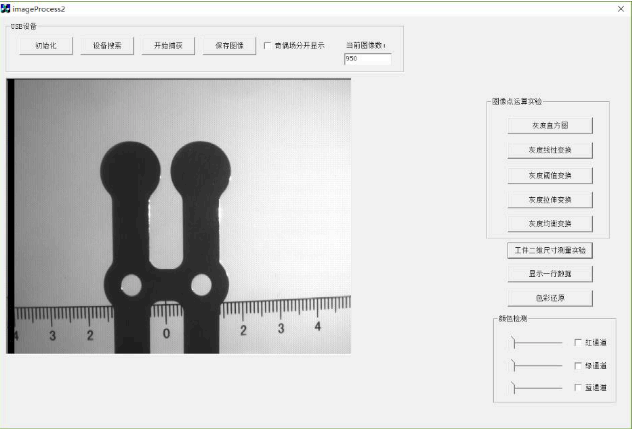
\includegraphics[scale=0.5]{4_1}
				\caption{工件安装示意及采集图例}
			\end{figure}
			上图中,可以看到采集到的图像左侧有一列 16 个像素的黑电平,这是因为本相机采用的是流水线 ADC,它需要 16 个周期的流水线建立时间。流水线 ADC 的优点是有良好的线性和低失调;可以同时对多个采样进行处理,有较高的信号处理速度;低功率;高精度;高分辨率。缺点是基准电路和偏置结构过于复杂;输入信号需要经过特殊处理,以便穿过数级电路造成流水延迟;对锁存定时的要求严格;对电路工艺要求很高,电路板上设计得不合理会影响增益的线性、失调及其它参数。
			\item 查看图片某一行数据,并思考图像明暗和灰度值之间的关系,分析图像边沿位置的灰度值特点。
			\begin{figure}[H]
				\centering
				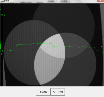
\includegraphics[scale=2]{4_2}
				\caption{图像明暗和灰度值之间的关系图}
			\end{figure}
			\item 点击保存按钮“保存图像”,将采集到的图像保存在磁盘上并在当前文件夹搜索image.bmp 文件,看看是否为刚刚保存的图像
			\item 
		\end{enumerate}
		\item 图像运算
		\begin{enumerate}[(a)]
			\item 将被测物体和标定尺子放置于夹持器上,依次点击初始化按钮、设备搜索按钮和开始捕获按钮,开始采集图像,调整相机镜头焦距,使获得的图像清晰,对比度高。
			\item 待图像清晰稳定后,点击停止捕获按钮“停止捕获”,得到一副清晰的图像。点击灰度直方图按钮“灰度”,在弹出的对话框中,先点击“显示原图”,再点击“显示灰度直方图”,查看图像直方图分布,并分析直方图分布和图像有什么关系。
			\begin{figure}[H]
				\centering
				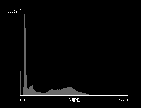
\includegraphics[scale=1.5]{4_3}
				\caption{灰度直方图}
			\end{figure}
			\item 按同样的方法查看对图像进行灰度线性变换,灰度阈值变换、灰度拉伸变换和灰度均衡变换。并分析各种变换后,图像的那些信息发生变化。
		\end{enumerate}
		\item 颜色处理(选做,无彩色面阵 CCD,按灰色颜色处理)
		\begin{enumerate}[(a)]
			\item 用USB 连接线将彩色面阵CCD相机与计算机的USB2.0 连接起来;打开计算机的电源开关,确定“面阵CCD 颜色识别实验”程序是否已经安装;
			\item 点击奇偶场分开显示,按照前面实验的要求采集一副清晰的三原色标准卡奇偶场相片,点击色彩还原按钮“色彩还原”获得一副彩色图像。
			\item 显示图片不同通道的图像,并分析哪种颜色在哪个通道灰度值比较大。
		\end{enumerate}
	\end{enumerate}

	\subsubsection{利用面阵 CCD 测量工件二维尺寸}
	\begin{enumerate}
		\item 将被测工件和标定尺放置于夹持器上,将面阵 CCD 相机接入电脑,调整相机镜
		头焦距,按照前面实验的方法,采集一副清晰的图像。
		\item 点击工件二维尺寸测量按钮,在弹出的对话框中先将采集到的图像显示出来。
		\item 点击相机标定按钮“相机标定”,对本系统进行标定,使像素和物体尺寸建立映射关系,选择点时需十分小心,标定结果的好坏直接导致测量数据准确与否。
		\item 标定完成后,点选圆半径按钮“圆半径”,在图像上鼠标左键点选被测工件上的特征圆圆心并拖至所测圆边圆外,然后点鼠标右键确定位置,得到被测圆的半径,
		\item 点击检测圆间距按钮,测量工件上两个圆圆心间距
		\item 点击检测平行线距离按钮“平行距离”,检测工件上两平行边的距离
		\item 对上述特征进行多次测量,并与游标卡尺的测量结果对比,分析误差原因。
		\begin{table}[H]
			\caption{圆半径}
			\centering
			\begin{tabular}{| c | p{2cm} | p{2cm} | p{2cm} | p{2cm} |}
				\hline
				编号 & 1 & 2 & 3 & 4 \\
				\hline
				游标卡尺测量值 & & & & \\
				\hline
				CCD测量值 & & & & \\
				\hline
				误差 & & & & \\
				\hline
			\end{tabular}
		\end{table}
	\begin{table}[H]
		\caption{圆间距}
		\centering
		\begin{tabular}{| c | p{2cm} | p{2cm} | p{2cm} | p{2cm} |}
			\hline
			编号 & 1 & 2 & 3 & 4 \\
			\hline
			游标卡尺测量值 & & & & \\
			\hline
			CCD测量值 & & & & \\
			\hline
			误差 & & & & \\
			\hline
		\end{tabular}
	\end{table}
\begin{table}[H]
	\caption{平行线距离}
	\centering
	\begin{tabular}{| c | p{2cm} | p{2cm} | p{2cm} | p{2cm} |}
		\hline
		编号 & 1 & 2 & 3 & 4 \\
		\hline
		游标卡尺测量值 & & & & \\
		\hline
		CCD测量值 & & & & \\
		\hline
		误差 & & & & \\
		\hline
	\end{tabular}
\end{table}
	\end{enumerate}
        
\subsection{实验原始数据}
实验原始数据记录表格如图所示。
\cpicn{0.2}{1}{实验数据记录表格。}
\cpicn{0.2}{2}{实验数据记录表格。}
\cpicn{0.2}{3}{实验数据记录表格。}
\cpicn{0.2}{4}{实验数据记录表格。}
\cpicn{0.2}{5}{实验数据记录表格。}
\cpicn{0.2}{6}{实验数据记录表格。}

\subsection{实验结束后的教师签名}
实验之后的教师签名如图~\ref{sign_1}~\ref{sign_2}所示。
\cpicn{0.3}{sign_1}{首页签名}
\cpicn{0.3}{sign_2}{实验记录之前的签名}

\subsection{实验中遇到的问题记录}
在角位移测量实验中,我们一开始发现激光无法在CCD感光部分上形成一个很窄的带,这是由于激光光源处未与透镜准直造成的,在适当调节激光光源与透镜的距离之后,输出的激光的发散角$\theta$就很小,这就造成了激光在线阵CCD上的发散距离
\beq
l = r\theta
\eeq
其中$r$为光走过的路程,而$l$为发散距离。在发散角很小的情况下,激光就在CCD上集中成一个很小的光斑,而采集到的信号就会变成一个尖锐的峰,如图所示。
\cpicn{0.2}{sharp}{\color{red} 调整好激光光源与透镜之间的距离之后,采集到的电信号是一个尖锐的峰,如果不作调节,会得到一个十分发散的图样。}
\newpage        
\section{分析与讨论}
\begin{tabular}{|p{8em}|p{8em}|p{8em}|p{8em}|}
	\hline 
	专业:     &Physics       &年级:      & 17     \\
	\hline
	姓名:& 徐昊霆 &学号:&17353071  \\
	\hline
	日期&     2019.9               & &  \\
	\hline	
	评分 & & 教师签名 & \\
	\hline
\end{tabular}

\subsection{线阵CCD驱动及其特性测量}
首先我们将不同的输出端口与示波器链接,得到了测试端子的频率。我们测量得到SH,RS,$\Phi 1$和$\Phi 2$的周期如下
\bea
T_{SH} &=& 6920 \SImus \\
T_{RS} &=& 1.390 \SImus \\
T_{\Phi 1} &=& 2.775 \SImus \\
T_{\Phi 2} &=& 2.780 \SImus
\eea
由测量我们可以看到,$\Phi 1$与$\Phi 2$的周期有如下关系
\beq
T_{\Phi 1}\simeq T_{\Phi 2}
\eeq
与仪器的工作时序图~\ref{time}对比可以得到,$\Phi 1$与$\Phi 2 $势是周期几乎相同,相位完全相反的,这与我们的测量一致。通过我们测量还发现
\bea
T_{SH} \simeq 2494 T_{\Phi 1}
\eea
对比工作时序图~\ref{time}可以发现,转移脉冲SH的周期确实是$\Phi 1 ,\Phi 2$周期的很多倍。相邻两个 SH 脉冲之间的时间就是像敏单元的感光时间,这里称为积分时间。RS 是复位输出级的复位脉冲,复位一次输出一个光脉冲信号。在实验中我们观察到
\beq
T_{RS} \simeq \frac{1}{2}T_{\Phi}
\eeq
这说明在驱动信号的一个周期内,RS复位两次,在很短的时间内输出两个光脉冲的信号。

\subsection{工件直径和角位移测量实验}
\subsubsection{工件直径的测量}
不论是测量工件的直径还是角位移,首先都需要进行标定--将像素点与空间中的实际距离联系起来。我们使用了实验室提供的标准的$\phi 10$工件(直径为$10\SImm$)进行标定,我们之后旋转了工件$\phi 10$,通过人为在图像上选择被挡住的临界点(实际操作中,选择电信号变化最快的那个点,大约为极大值和极小值的中点),使用之前的标定数据,我们很容易就计算得到我们所测量的旋转之后的工件直径(或者说,是测量了旋转之后的工件直径与之前工件直径的比值更为合适)
\beq
d = \frac{\sum_{i=1^{3}} d_i}{3} = 1.0509 \SIcm
\eeq
另外,使用游标卡尺测量得到工件的直径为$d = 10.00\SIcm$,可见实验室提供的工件十分标准,测量得到的平均值绝对误差(测量值-真值)为
\beq
\sigma_{d} = \sqrt{\frac{\sum_{i=1}^{3} (d_i - d_{\rm real})^2}{3\times 2}} = 0.015 \SIcm
\eeq
这里我们因为误差的第一有效位数是1,所以按照误差分析理论~\cite{error},可以多保留一位。所以最终测量结果可以表述为
\beq
d = \left(1.059 \pm 0.015\right) \SIcm
\eeq
可见平均值的标准差并不包括真值。测量值大概有$6\%$的误差。这一误差并不是由于前面所述的随机误差得到的,而是由于工件的切面不是一个严格的圆造成的。我们在这里把工件的切面形状近似为椭圆。在二维平面上,椭圆方程为
\beq
\frac{x^2}{a^2} + \frac{y^2}{b^2} = 1
\eeq
椭圆的离心率定义为$e = c/a$,其中$c$为椭圆的焦距。离心率是衡量椭圆被压扁程度的参数。离心率为0意味着椭圆退化为圆,离心率为1意味着椭圆退化为一条直线。在本实验中,我们可以给出工件切面离心率的下限
\beq
e\ge \frac{\sqrt{b^2 - a^2}}{a} \simeq 0.035
\eeq
可见工件还是有了一定的变形。

通过同样的原理,仍然使用实验室提供的标准$\phi 10$滚针的标定数值,测得$\phi 12$滚针的平均值为
\beq
d = \frac{\sum_{i=1^{3}} d_i}{3} = 1.215 \SIcm
\eeq
相比于$\phi 10$滚针,$\phi 12$滚针的直径就没有$1.2\SIcm$那么精准,使用游标卡尺得到$\phi 12$滚针的直径为
\beq
d = 1.210 \SIcm
\eeq
请注意上面的结果是由游标卡尺得到的。通过测量值减去真值(这里的真值认为是从游标卡尺得到的),按照误差分析公式(见参考文献~\cite{error})我们得到测量平均值的标准误差为
\beq
\sigma_{d} = \sqrt{\frac{\sum_{i=1}^{3} (d_i - d_{\rm real})^2}{3\times 2}} =0.007 \SIcm
\eeq
由此可见,与前面的$\phi 10$工件相比较,$\phi 12$工件更加均匀,离心率更小,更加接近圆柱体。
\subsubsection{角位置测量实验}
在角位移测量实验中,我们一开始发现激光无法在CCD感光部分上形成一个很窄的带,这是由于激光光源处未与透镜准直造成的,在适当调节激光光源与透镜的距离之后,输出的激光的发散角$\theta$就很小,这就造成了激光在线阵CCD上的发散距离
\beq
l = r\theta
\eeq
其中$r$为光走过的路程,而$l$为发散距离。在发散角很小的情况下,激光就在CCD上集中成一个很小的光斑,而采集到的信号就会变成一个尖锐的峰。

在实验中,我们记录下位置1和位置2的像素位置,通过乘以像素对应的距离大小$14\SImum$,我们得到光线转过的角度为
\beq \label{angular}
\theta = \frac{\Delta \psi \times 14\SImum}{l}
\eeq
其中$\Delta\psi$为像素之差,$l$为反射镜中心到CCD中心的距离。在实验中我们测量得到
\beq
l = 14.55\SIcm
\eeq
这样我们可以通过式~\ref{angular}来知道光线旋转角度的弧度值,为了得到反射镜旋转的角度,我们将式~\ref{angular}得到的角度除以2并换算为弧度
\beq \label{mirror}
\varphi =  \frac{1}{2}\times \frac{\Delta \psi \times 14\SImum}{14.55\SIcm}\times \frac{180^{\circ}}{\pi}
\eeq
在实验中,我们将反射镜旋转不同的角度,记录下反射镜实际旋转的角度,同时记录下尖锐的峰最高处像素点的差,使用公式~\ref{angular},得到三次测量\textbf{光线旋转角度}(以弧度为单位)
\bea
\theta_1 &=& 0.813 \rad \\
\theta_2 &=& 1.177 \rad \\
\theta_3 &=& 1.116 \rad
\eea
进而通过式~\ref{mirror}换算得到镜子旋转的角度为
\bea
\varphi_1 &=& 23.29 ^{\circ}\\
\varphi_2 &=& 33.72 ^{\circ}\\
\varphi_3 &=& 31.97 ^{\circ}
\eea
与实际上反射镜旋转过的角度进行比较,得到本次测量的相对误差
\bea
\left(\frac{\Delta \varphi}{\varphi}\right)_1 &=& 0.0126\\
\left(\frac{\Delta \varphi}{\varphi}\right)_2 &=& 0.0082\\
\left(\frac{\Delta \varphi}{\varphi}\right)_3 &=& 0.0102
\eea
可见测量结果十分精确。但是请注意!我们是严格使用讲义的方法得到的,也就是式~\ref{mirror},但实际过程中我们移动的角度并不是一个小量,实际上应该使用下面的式子进行计算
\beq
\Delta \psi \times 14\SImum = 2l \sin \frac{\theta}{2}
\eeq
在实际操作中,我们测量的实际上是光线的波前所在的圆弧在CCD平面上的投影,因此我们对于光线波前圆弧长度的测量存在如下误差
\beq
\delta = l\left(\theta - 2\sin\frac{\theta}{2}\right)
\eeq
将上面的式子进行泰勒展开,保留到11阶
\beq
\theta - 2\sin\frac{\theta}{2} \simeq\frac{2}{3!}\left(\frac{\theta}{2}\right)^3-\frac{2}{5!}\left(\frac{\theta}{2}\right)^5+\frac{2}{7!}\left(\frac{\theta}{2}\right)^7-\frac{2}{9!}\left(\frac{\theta}{2}\right)^9+ \frac{2}{11!}\left(\frac{\theta}{2}\right)^{11}
\eeq
由上面的公式我们计算得到,对于弧度为1,误差大概为
\beq
\delta \simeq l \times0.05
\eeq
可见,这里系统误差大约为$0.05\times l$,从而引起的角度的误差大约为$0.025\rad$。
\subsection{面阵CCD图像采集、运算和颜色处理}
首先我们按照实验讲义组装了仪器,首先得到一张原始图像如图~\ref{CCD/原图}所示。
\cpicn{0.5}{CCD/原图}{原始图像}
然后我们点击软件上的显示灰度的数值,得到其中的而一行数据如图~\ref{CCD/一行数据}所示。
\cpicn{0.5}{CCD/一行数据}{原图上灰度的一行数据。}
从上面一行数据的图像我们可以发现,在黑色的地方,像素点的灰度数据为0,而在比较白的地方,像素点的灰度数据大概为255,但是在图像上的白的地方实际上不是完全的稳定在255,而是由于环境灯光的影响,在255处有小幅度波动。

我们点击软件上的灰度线性变换按钮。这种变换的原理非常简单,即采集了各个像素点的灰度数据,然后对其进行线性的变换。回想在前面的章节中,我们写出了线性灰度变换函数
\beq
f(x) = f_A \, x +f_B
\eeq
为了取得明显的变换效果,我们取如下的参数设置
\bea
f_A &=& -1\\
f_B &=& 225
\eea
很显然,如果这样做线性变换,则全黑变为全白,全白变为全黑,实验中我们得到的图像如图~\ref{CCD/灰度线性变换}所示,显然符合我们的预期。
\cpicn{0.5}{CCD/灰度线性变换}{进行了灰度线性变换得到的数据。}

同样地,我们期望探索更多的变换方式,接下来要展示的是灰度阈值变换,灰度阈值变换就是设定一个阈值,将小于阈值的直接变为纯白(灰度为0),将大于阈值的点全部变为纯黑(灰度为255)。在实验中,我们设定灰度的阈值为90,变换后得到的图像如图~\ref{CCD/灰度阈值变换}所示。由图像我们可以看到,在H型工件的边缘位置由于反光的缘故,有一些像素点虽然在原图上看起来比较黑,但是实际上灰度还没有达到我们设定的阈值。所以在变换之后的图上我们看到有一些点显示为全白。
\cpicn{0.5}{CCD/灰度阈值变换}{将原图进行灰度阈值变换后得到的图像}

对于灰度拉伸变换,灰度拉伸变换与灰度线性变换类似,只不过是一个分段函数。我们得到的灰度的拉伸变换如图所示。
\cpicn{0.5}{CCD/灰度拉伸变换}{灰度拉伸变换之后得到的图像。}

灰度均衡变换,灰度均衡变换有时也称直方图均衡变换,它能使输入图像转换为
在新图像每一灰度级上都有相同的像素点数的输出图像。灰度均衡变换的原理式如下
\beq
A[a] = \left(\sum_{i = 0}^a  N[i]\right)\times 225 /(H\cdot W)
\eeq
式中 $a$ 为原图像像素灰度值(0-255),经过灰度均衡运算 $a$ 的值变为灰度均衡值 $A,N$ 为原图像各灰度值对应的像元数量,$H$ 为图像的高度(单位是像元数),W 为图像的宽度(单位是像元数)。例如原图像像元灰度值为 20 的像素点,经灰度均衡变换后,灰度变为
\beq
A[20] = \left(\sum_{i = 0}^{20}  N[i]\right)\times 225 /(H\cdot W)
\eeq
经过灰度均衡后,图像的对比度大大提高,转换后图像的灰度分布也趋于均匀。经过灰度均衡变换得到的图像如图所示。
\cpicn{0.5}{CCD/灰度均衡变换直方图}{经过灰度均衡变换得到的图样。}

之后我们切换为彩色的一面,点击软件上奇偶场分开显示,得到三原色在奇偶场中的图样如图~\ref{CCD/三原色奇偶场}所示。
\cpicn{0.5}{CCD/三原色奇偶场}{三原色在奇偶场分开显示的图样。}

与灰度的直方图类似,我们使用的软件的任何原色都是由红绿蓝三组颜色构成的,对于每一个颜色,都有一个表征这个点颜色组分的值,通过读取每一个像素点的值来进行三原色还原得到如图~\ref{CCD/三原色色彩还原}所示的图像。在现代人的眼光中,这个图样并没有很好地还原这张图像,在现代的计算机中,我们使用更多的颜色组分。
\cpicn{0.5}{CCD/三原色色彩还原}{使用CCD软件得到的三原色色彩还原图像。}

如果我们只打开三原色通道的红、绿、蓝通道,这样只有绿色的部分才可以在绿通道显示,而其他的颜色就会显示为黑色。红、绿、蓝三个通道处理过后的图样如图~\ref{CCD/红通道}~\ref{CCD/绿通道}~\ref{CCD/蓝通道}所示。
\cpicn{0.5}{CCD/红通道}{只有红通道时得到的图像。}
\cpicn{0.5}{CCD/绿通道}{只有绿通道时得到的图像。}
\cpicn{0.5}{CCD/蓝通道}{只有蓝通道时得到的图像。}

\subsection{利用面阵CCD测量工件二维尺寸}
首先,我们使用光屏上的标准尺进行标定,然后我们就可以使用软件上的选择工具,自动来匹配、测量圆半径、平行线间距等。测量结果如图~\ref{CCD/平行间距}~\ref{CCD/圆间距}~\ref{CCD/圆半径}。
\cpicn{0.5}{CCD/平行间距}{使用面阵CCD得到的两条平行线平行间距的结果。}
上面是记录的图像,与游标卡尺测量结果的比对在实验原始表格中,在那里我们计算了误差,可见测量相当精确。
\cpicn{0.5}{CCD/圆间距}{使用面阵CCD得到的两个圆间距的结果。}
上面是记录的图像,与游标卡尺测量结果的比对在实验原始表格中,在那里我们计算了误差,可见测量相当精确。
\cpicn{0.5}{CCD/圆半径}{使用面阵CCD得到的圆半径的测量结果。}
上面是记录的图像,与游标卡尺测量结果的比对在实验原始表格中,在那里我们计算了误差,可见测量相当精确。
\subsection{实验报告思考题}
\begin{enumerate}[(1)]
\item 请解释转移脉冲SH在线阵CCD中的作用。
\cpicn{0.5}{time}{TCD1208AP 工作时序图}
工作时序图如图~\ref{time}所示,当SH 高电平来到时,$\Phi 1$为高电平,$\Phi 2$为低电平($\Phi 1$,$\Phi 2$ 相互为互补时序脉冲)。CCD 模拟转移寄存器中所有 $\Phi 1$ 电极下均形成深势阱,同时 SH 的高电平使 $\Phi 1$ 电极下的深势阱与
MOS 电容存储势阱(转移栅)沟通,MOS 电容中的信号电荷包通过转移栅转移到模拟移位寄存器的 $\Phi 1$电极下的势阱中。当 SH 由高变低时,SH 低电平形成势垒,使 MOS 电容与 $\Phi 1$电极隔离。当 SH 由高变低时,SH 低电平形成势垒,使 MOS 电容与 $\Phi 1$电
极隔离。而后,$\Phi 1$与 $\Phi 2$交替变化,模拟移位寄存器在 $\Phi 1$ 与 $\Phi 2$ 脉冲的作用下驱使 $\Phi 1$
电极下势阱中的信号电荷向左移动,并经输出电路由 OS 电极输出。

\item 解释为什么修改驱动频率和积分时间会导致CCD相机输出信号产生影响?
  
  驱动频率影响输出信号的频率,积分时间影响帧速率。积分时间的改变本质上是通过增加或减少驱动脉冲来实现的。驱动脉冲频率上限受电荷自身转移时间限制,当工作频率升高时,若电荷本身从一个电极转移到另一个电极所需要的时间 t 大于驱动频率使其转移的时间 T/3,那么,信号电荷跟不上驱动脉冲的变化,将会使转移效率大大下降。SH 脉冲在高电平时沟通像敏单元和模拟转移寄存器,使像敏单元中的光电子转移到模拟转移寄存器。相邻两个 SH 脉冲之间的时间就是像敏单元的感光时间,这里称为积分时间。模拟转移寄存器中的光电荷的输出时间应该小于
积分时间才能保证光电信号的完整。

\item 如果输入到线阵CCD光敏面上的光太强或者积分时间太长,使CCD器件工作在饱和状态,此时线阵CCD输出信号有何特点?

  此时线阵CCD的输出信号就会超出仪器所能显示的最大值,而且不能分辨光的相对强弱 。
  
\item 如果图像为全黑或全白,则对应的灰度值应该是多少?
根据我们实验得到的灰度直方图,可以发现,当图像为全黑时,对应的灰度值应该是0,如果图像为全白,对应的灰度值为255。  
\item 为什么直方图均衡化能有效增强图像?

  灰度均衡变换,灰度均衡变换有时也称直方图均衡变换,它能使输入图像转换为
在新图像每一灰度级上都有相同的像素点数的输出图像。灰度均衡变换的原理式如下
\beq
A[a] = \left(\sum_{i = 0}^a  N[i]\right)\times 225 /(H\cdot W)
\eeq
式中 $a$ 为原图像像素灰度值(0-255),经过灰度均衡运算 $a$ 的值变为灰度均衡值 $A,N$ 为原图像各灰度值对应的像元数量,$H$ 为图像的高度(单位是像元数),W 为图像的宽度(单位是像元数)。例如原图像像元灰度值为 20 的像素点,经灰度均衡变换后,灰度变为
\beq
A[20] = \left(\sum_{i = 0}^{20}  N[i]\right)\times 225 /(H\cdot W)
\eeq
经过灰度均衡后,图像的对比度大大提高,转换后图像的灰度分布也趋于均匀。
\item 白色的图片在各个不同的通道灰度值有什么特点?
  白色的图片不论在哪个通道,灰度值一定为最大(255)。
\end{enumerate}



\bibliographystyle{siam}
\bibliography{cites}
\end{document}
